\section{Simulações} % Seções são adicionadas para organizar sua apresentação em blocos discretos, todas as seções e subseções são automaticamente exibidas no índice como uma visão geral da apresentação, mas NÃO são exibidas como slides separados.

%----------------------------------------------------------------------------------------

\begin{frame}{\textit{PE Model}: Processo de plotagem}

Dada a seleção do modelo, o seguinte processo é realizado:

\begin{enumerate}
    \item Seleção de constantes e condições iniciais
    \item Método de discretização (RK4)
    \item Plotagem
\end{enumerate}
\end{frame}


%----------------------------------------------------------------------------------------
\begin{frame}[fragile]

\frametitle{\textit{PE Model}: Seleção de constantes}
    
    \begin{python}
vetor_a = [1, 1, 3]
vetor_b = [
    0.5 * (vetor_a[0] - vetor_a[1] - vetor_a[2]),
    0.5 * (vetor_a[1] - vetor_a[2] - vetor_a[0]),
    0.5 * (vetor_a[2] - vetor_a[0] - vetor_a[1]),
]
c = math.sqrt(3/4)

f_inv = 10800
vetor_h = [-1, 0, 0]
vetor_f = [0.1, 0, 0]
g_0 = 8
kappa_0 = 1 / 48
nu_0 = kappa_0
    \end{python}
\end{frame}

%----------------------------------------------------------------------------------------
\begin{frame}[fragile]

\frametitle{\textit{PE Model}: Condições iniciais - padrão}
Primeira condição inicial, é a dada por padrão e tem o intuito de reproduzir a figura 1 do artigo.    
    \begin{python}
# Condições iniciais - dia 01
x0 = [0.1, 0, 0]
y0 = [0.1, 0, 0]
z0 = [0.1, 0, 0]
    \end{python}
\end{frame}

%----------------------------------------------------------------------------------------

\begin{frame}{COndição de Hardley}
    
\end{frame}


%----------------------------------------------------------------------------------------
\begin{frame}[fragile]

\frametitle{\textit{PE Model}: Condições iniciais - Hardley 01}
A presente condição reproduz as condições da circulação de Hardley de acordo como \cite{gent1982}:
    \begin{python}
# Condição Hardley 01
y1 = (vetor_f[1] / vetor_a[1] * nu_0 * (1 + vetor_a[1] * g_0 + nu_0**2 * vetor_a[1] ** 2))
z1 = (1 + nu_0**2 * vetor_a[1] ** 2) * y1
x1 = -nu_0 * vetor_a[1] * y1

    
x_hardley_inicial = [x1, 0, 0]
y_hardley_inicial = [y1, -(10 ** (-5)), 0]
z_hardley_inicial = [z1, 10 ** (-5), 0]
    \end{python}
\end{frame}


%----------------------------------------------------------------------------------------
\begin{frame}[fragile]

\frametitle{\textit{PE Model e QG Model}: Condições iniciais - Hardley 02}
A presente condição reproduz as condições da circulação de Hardley de acordo com \cite{lorenz1980}
    \begin{python}
x_hardley02_inicial = [-0.01111, 0, 0]
y_hardley02_inicial = [0.53331, 0, 0]
z_hardle02_inicial = [0.53354, 0, 0]
    \end{python}

Equivalente a seguinte condição do QG Model:
    \begin{python}
y0 = [0.53333, 0, 0]
    \end{python}
\end{frame}

%----------------------------------------------------------------------------------------

\begin{frame}{Método de discretização RK4}
    
\end{frame}

%----------------------------------------------------------------------------------------



\begin{frame}{\textit{PE Model}: Resultados condição inicial padrão}
   \begin{figure}
       \centering
       \begin{subfigure}[b]{0.45\textwidth}
           \centering
           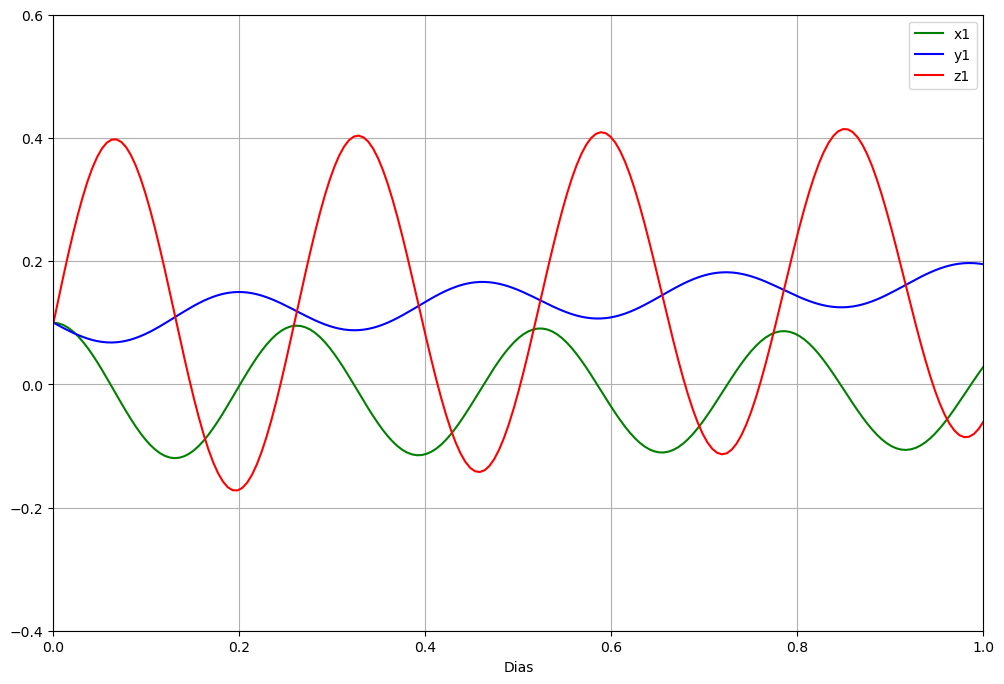
\includegraphics[width=\textwidth]{img/p01d01.png}
           \caption{Condição padrão - reprodução}
           \label{fig:p01d01}
       \end{subfigure}
       \hfill
       \begin{subfigure}[b]{0.45\textwidth}
           \centering
           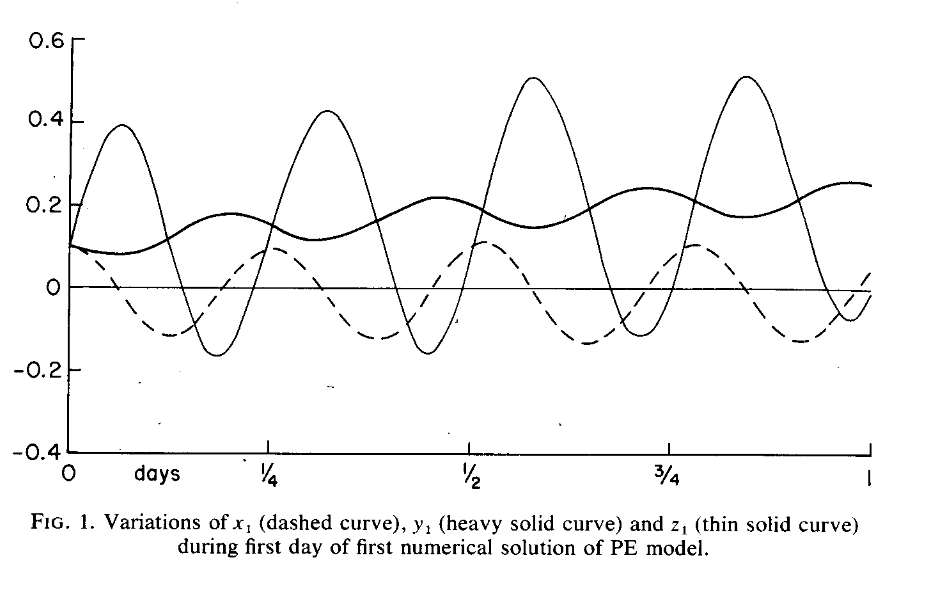
\includegraphics[width=\textwidth]{img/p01d01rel.png}
           \caption{Condição padrão - artigo}
           \label{fig:p01d01rel}
       \end{subfigure}
   \end{figure}
\end{frame}

%----------------------------------------------------------------------------------------

\begin{frame}{\textit{PE Model}: Resultados condição inicial padrão}
   \begin{figure}
       \centering
       \begin{subfigure}[b]{0.45\textwidth}
           \centering
           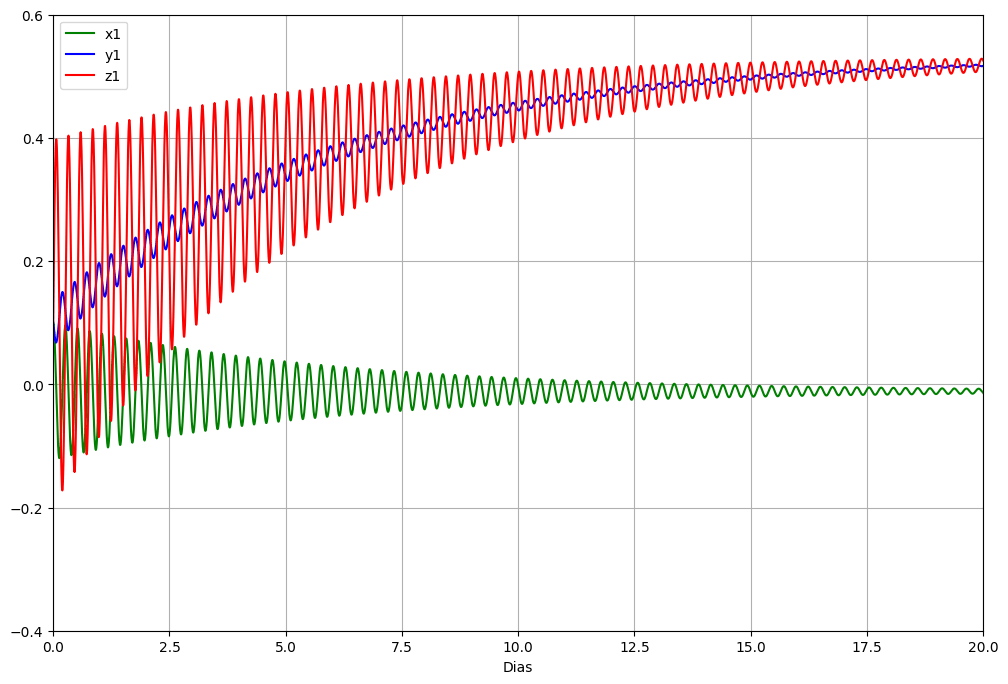
\includegraphics[width=\textwidth]{img/p01d20.png}
           \caption{Condição padrão - 20 dias}
           \label{fig:p01d20}
       \end{subfigure}
       \hfill
       \begin{subfigure}[b]{0.45\textwidth}
           \centering
           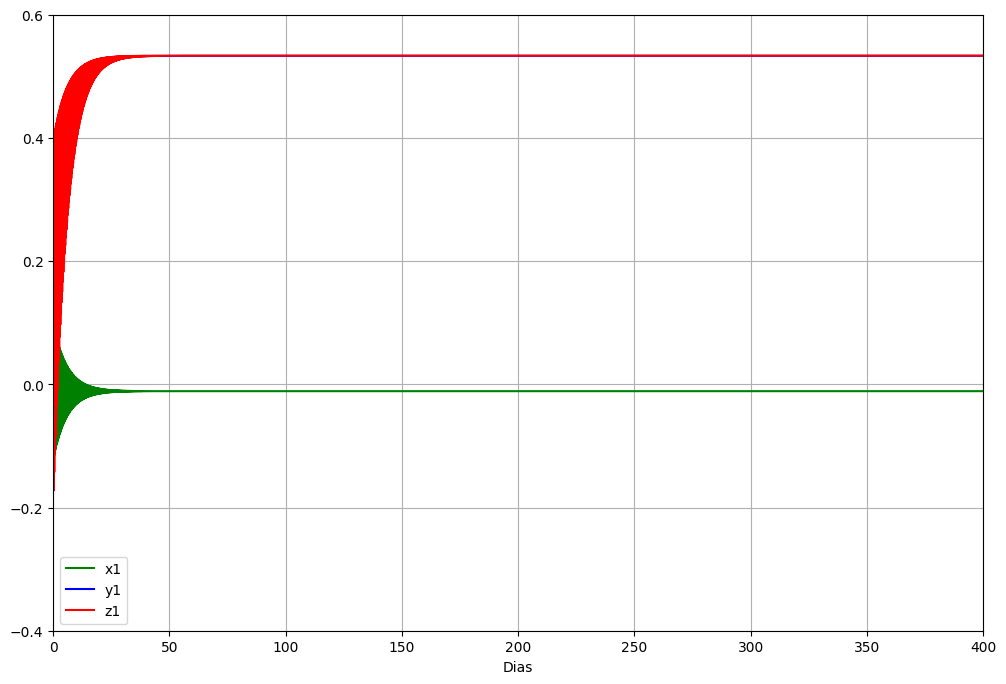
\includegraphics[width=\textwidth]{img/p01d400.png}
           \caption{Condição padrão - 400 dias}
           \label{fig:p01d400}
       \end{subfigure}
   \end{figure}
\end{frame}


%----------------------------------------------------------------------------------------

\begin{frame}{\textit{PE Model}: Resultados para condição de Hardley 01}
   \begin{figure}
       \centering
       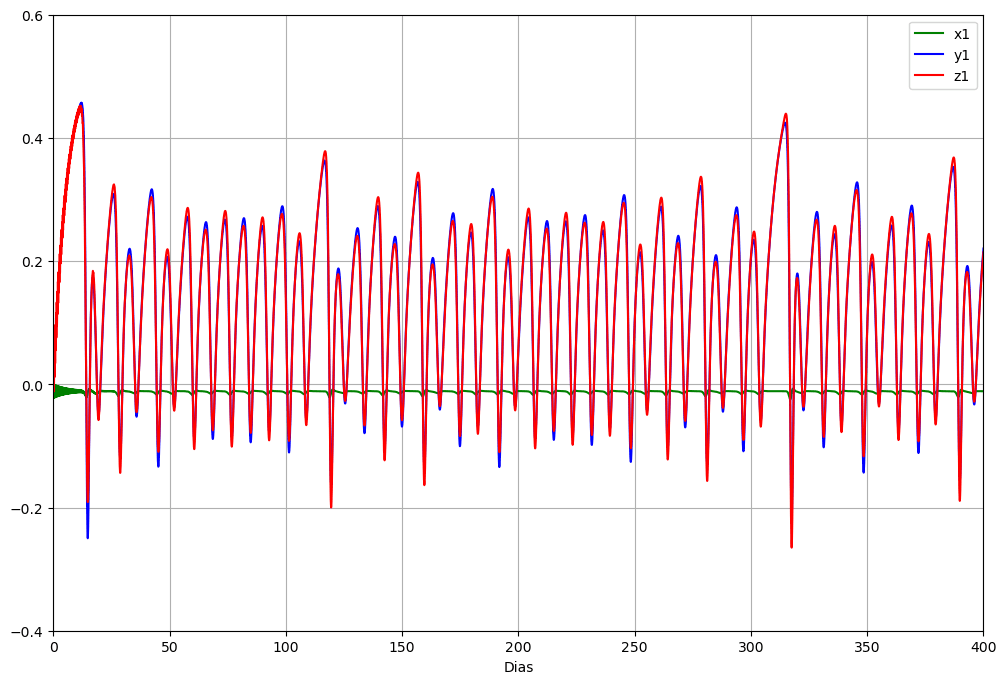
\includegraphics[width=0.5\textwidth]{img/p02d260.png}
       \caption{Hardley 01 - 260 dias}
       \label{fig:p02}
   \end{figure}
\end{frame}


%----------------------------------------------------------------------------------------

\begin{frame}{\textit{PE Model}: Resultados para condição de Hardley 01}
   \begin{figure}
       \centering
           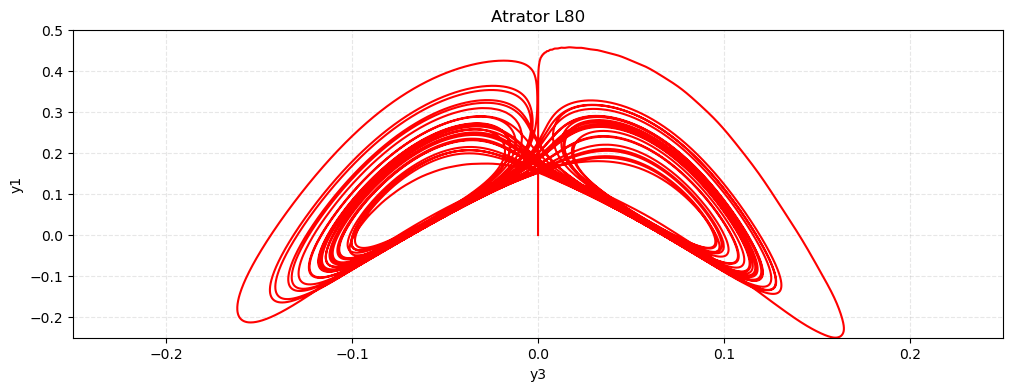
\includegraphics[width=0.8\textwidth]{img/p02y3y1.png}
       \caption{Hardley 01 - Projeção $y_3 \times y_1$}
       \label{fig:p02y3y1}
   \end{figure}
\end{frame}

%----------------------------------------------------------------------------------------

\begin{frame}{\textit{PE Model}: Resultados para condição de Hardley 01}
   \begin{figure}
       \centering
       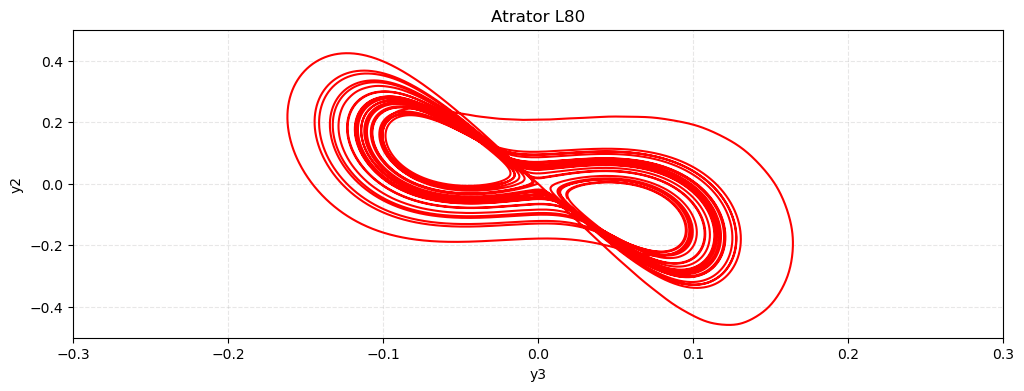
\includegraphics[width=0.8\textwidth]{img/p02y3y2.png}
       \caption{Hardley 01 - Projeção $y_3 \times y_2$}
       \label{fig:p02y3y2}
   \end{figure}
\end{frame}

%----------------------------------------------------------------------------------------

\begin{frame}{\textit{PE Model}: Resultados para condição de Hardley 01}
   \begin{figure}
       \centering
       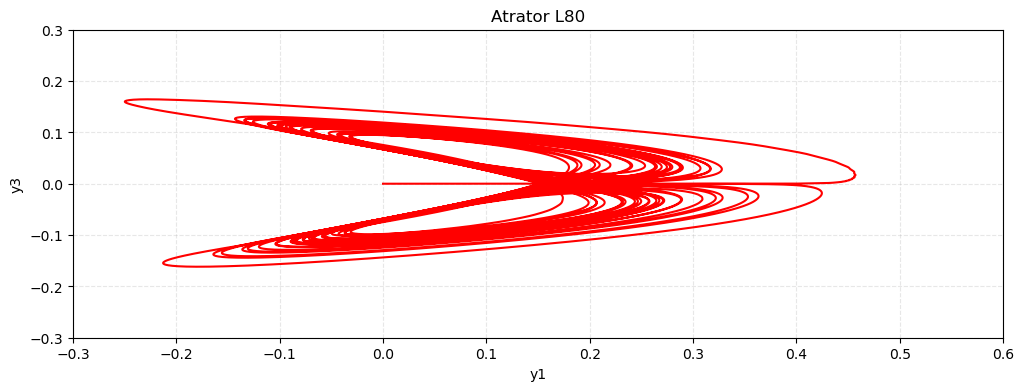
\includegraphics[width=0.8\textwidth]{img/p02y1y3.png}
       \caption{Hardley 01 - Projeção $y_1 \times y_3$}
       \label{fig:p02y1y3}
   \end{figure}
\end{frame}

%----------------------------------------------------------------------------------------

\begin{frame}{\textit{PE Model} e \textit{QG Model}: Resultados para a condição de Hardley 02}
   \begin{figure}
       \centering
       \begin{subfigure}[b]{0.45\textwidth}
           \centering
           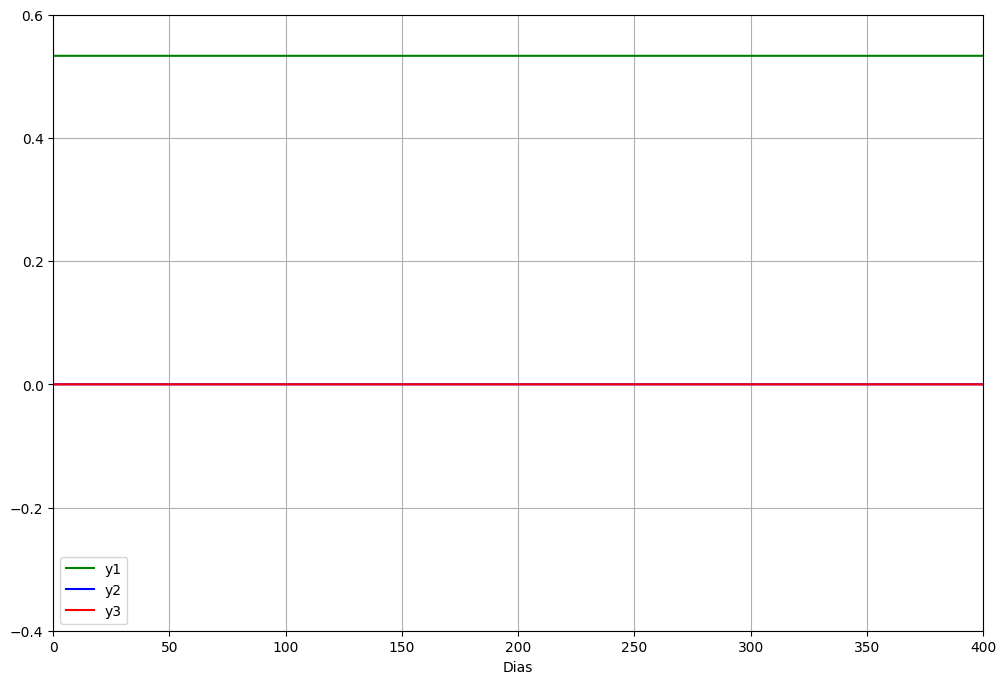
\includegraphics[width=\textwidth]{img/p03d400pe.png}
           \caption{Condição de Hardley 02 - 400 dias\\ (PE Model)}
           \label{fig:p03d400pe}
       \end{subfigure}
       \hfill
       \begin{subfigure}[b]{0.45\textwidth}
           \centering
           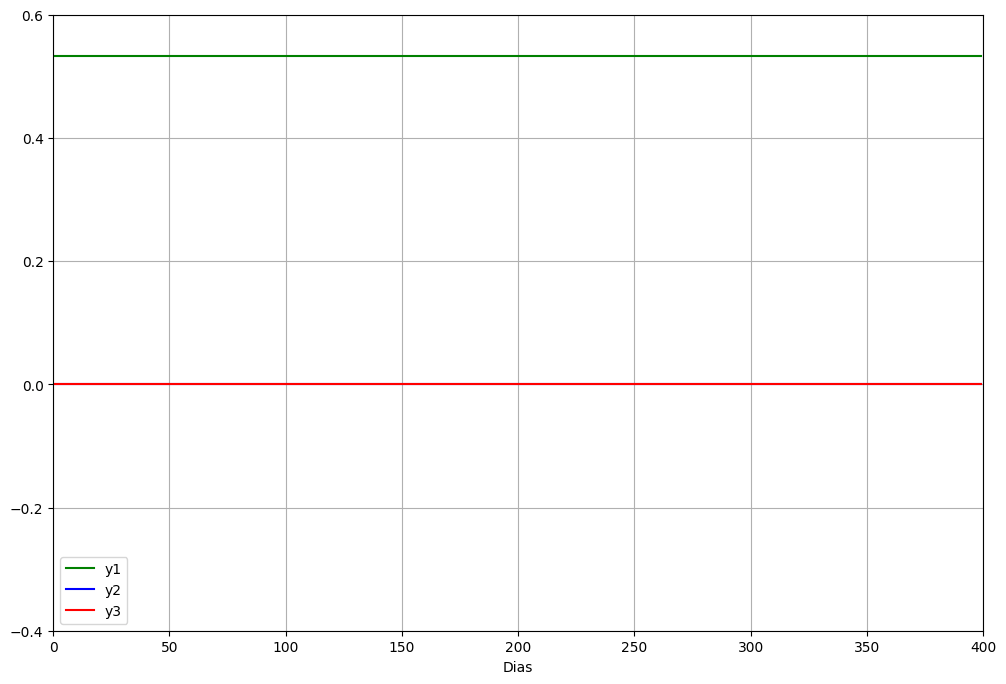
\includegraphics[width=\textwidth]{img/p03d400qg.png}
           \caption{Condição de Hardley 02 - 400 dias\\ (QG Model)}
           \label{fig:p03d400qg}
       \end{subfigure}
   \end{figure}
\end{frame}

